\documentclass[11pt,twocolumn,a4paper]{article}
\usepackage{amsmath}
\usepackage{amssymb}
\usepackage{graphicx}
\usepackage{booktabs}
\usepackage{hyperref}
\usepackage{float}
\usepackage{geometry}
\usepackage{xcolor}
\usepackage{microtype}
\usepackage{titlesec}
\usepackage{caption}
\usepackage{abstract}
\usepackage{fancyhdr}
\usepackage{tikz}
\usetikzlibrary{shapes.geometric, arrows, positioning}

% Page geometry matching the GSMI/Springer style
\geometry{
    a4paper,
    left=15mm,
    right=15mm,
    top=22mm,
    bottom=22mm,
    footskip=10mm
}

\hypersetup{
    colorlinks=true,
    linkcolor=blue,
    filecolor=magenta,      
    urlcolor=cyan,
    pdftitle={Reproducible and Lossless GIS Feature Extraction Pipeline},
    pdfpagemode=FullScreen,
}

\raggedbottom

% Header/Footer configuration
\pagestyle{fancy}
\fancyhf{}
\fancyhead[L]{\textsf{GSMI-UM6P}}
\fancyhead[R]{\textsf{Phase 3 Technical Report}}
\fancyfoot[C]{\thepage}
\renewcommand{\headrulewidth}{0.4pt}
\renewcommand{\footrulewidth}{0pt}

% Section style
\titleformat{\section}{\large\bfseries\sffamily}{\thesection}{1em}{}
\titleformat{\subsection}{\normalsize\bfseries\sffamily}{\thesubsection}{1em}{}

\renewenvironment{abstract}{%
    \small\sffamily
    \noindent\textbf{Abstract}\quad
}{%
    \vspace{0.4cm}
}

\begin{document}

\twocolumn[
    \begin{@twocolumnfalse}
        \begin{center}
            {
\includegraphics[width=0.4\textwidth]{logo.png}}
        \end{center}
        \vspace{0.4cm}
        
        {\Huge\bfseries\sffamily Reproducible and Lossless GIS Raster Feature Extraction: A Production-Grade Pipeline for Geoheritage Modeling\par}
        \vspace{0.6cm}
        
        {\large\textbf{EL GORRIM Mohamed}\par}
        {\small\sffamily AI Research Intern, Geology and Sustainable Mining Institute (GSMI), Mohammed VI Polytechnic University (UM6P), Ben Guerir, Morocco\par}
        \vspace{0.4cm}
        {\small\sffamily\textbf{Prepared for:} Dr. Ismail BEN AMAR, Sanae EL HARCHE, and Mohamed EL OUALI\par}
        \vspace{0.6cm}
        
        \begin{abstract}
        In geosite spatial modeling, translating geographical maps (rasters) into numeric tabular matrices for machine learning is highly prone to spatial distortion and class-code degradation. GIS layouts are often exported as visual RGB images with anti-aliasing artifacts, which introduces decimal interpolation errors when standard bilinear sampling is applied. This report documents the implementation of a generic, production-grade spatial feature extraction tool designed to resolve these data integrity challenges. The tool integrates Rasterio for raw raster matrix parsing, Pyproj for WGS84 to Morocco Sahara Lambert (EPSG:26191) coordinate transformations, OpenCV for geodesic distance scaling, and SciPy KDTree color lookup indices. The pipeline ensures 100\% lossless retrieval of categorical class IDs (Soil, LULC, Geology) and precise continuous metrics (Elevation, Slope, and infrastructure road distances) with sub-second processing speeds. This architecture provides a fully decoupled, reproducible pipeline suitable for any GIS-to-CSV extraction workflow.
        \end{abstract}
        
        \noindent\textbf{Keywords} GIS Extraction $\cdot$ Coordinate Transformation $\cdot$ Lossless Data Integrity $\cdot$ KDTree Color Decoding $\cdot$ Morocco Sahara Lambert
        \vspace{0.8cm}
    \end{@twocolumnfalse}
]

\section{Introduction}
Spatial predictive modeling of geological heritage (geosites) requires the fusion of tabular field coordinate databases with physical spatial rasters, such as Digital Elevation Models (DEM), Soil classifications, and Land Use/Land Cover (LULC) maps. 

However, in standard academic workflows, researchers face two major technical hurdles when converting GIS maps to tabular data:
\begin{enumerate}
    \item \textbf{Categorical Data Corruption}: Warping, reprojecting, or querying rasters using standard bilinear interpolation introduces intermediate fractional codes (e.g., querying Soil Class 2 and 3 and obtaining 2.5), which destroys the categorical integrity.
    \item \textbf{Visual RGB Layout Rasterization}: Many thematic layers are exported from ArcGIS/QGIS as visual RGB images (PNG/GIF) rather than single-band integer arrays. The borders between classes contain blended pixels due to anti-aliasing, leading to hundreds of false color IDs.
\end{enumerate}

To address these concerns, Phase 3 of this work establishes a general-purpose, production-grade command-line tool (CLI) named \texttt{general\_extractor.py}. This tool decouples the feature extraction pipeline from the specific study area, enabling lossless GIS-to-CSV translation for any coordinate coordinates database and arbitrary stack of rasters.

\section{Methodology and Computational Tools}

The technical architecture of the extraction pipeline is structured as a five-stage processing flow, depicted in Figure~\ref{fig:flowchart}.

\begin{figure}[H]
    \centering
    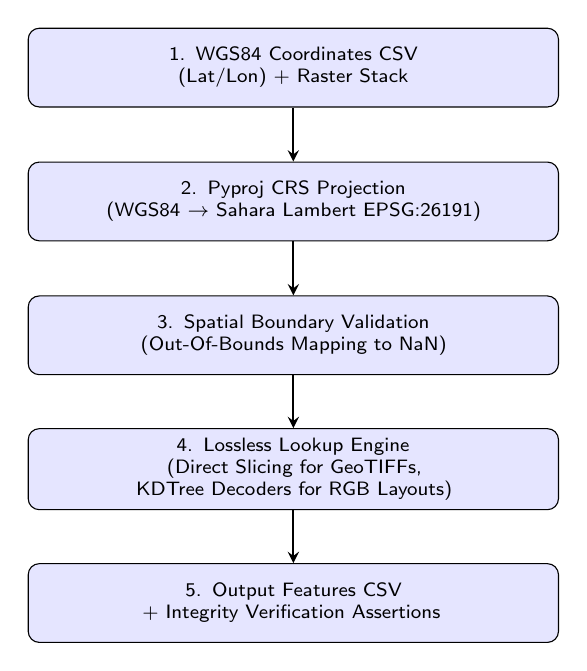
\begin{tikzpicture}[node distance=1.5cm, auto]
        \tikzstyle{block} = [rectangle, draw, fill=blue!10, text width=6.5cm, text centered, rounded corners, minimum height=1.0cm, font=\sffamily\scriptsize]
        \tikzstyle{line} = [draw, -stealth, thick]
        
        % Nodes
        \node [block] (input) {1. WGS84 Coordinates CSV \\ (Lat/Lon) + Raster Stack};
        \node [block, below of=input, yshift=-0.2cm] (proj) {2. Pyproj CRS Projection \\ (WGS84 $\rightarrow$ Sahara Lambert EPSG:26191)};
        \node [block, below of=proj, yshift=-0.2cm] (bounds) {3. Spatial Boundary Validation \\ (Out-Of-Bounds Mapping to NaN)};
        \node [block, below of=bounds, yshift=-0.2cm] (lookup) {4. Lossless Lookup Engine \\ (Direct Slicing for GeoTIFFs, \\ KDTree Decoders for RGB Layouts)};
        \node [block, below of=lookup, yshift=-0.2cm] (output) {5. Output Features CSV \\ + Integrity Verification Assertions};
        
        % Paths
        \path [line] (input) -- (proj);
        \path [line] (proj) -- (bounds);
        \path [line] (bounds) -- (lookup);
        \path [line] (lookup) -- (output);
    \end{tikzpicture}
    \caption{Lossless feature extraction pipeline architecture.}
    \label{fig:flowchart}
\end{figure}

\subsection{Coordinate Projection (Pyproj)}
To ensure metric spatial resolution is preserved across Morocco, coordinates are reprojected from WGS84 (\texttt{EPSG:4326}) to the official Morocco Sahara Lambert system (\texttt{EPSG:26191}) using a Pyproj coordinate Transformer:
\begin{equation}
    (x_{\text{proj}}, y_{\text{proj}}) = \mathcal{T}_{\text{WGS84}\rightarrow\text{Lambert}}(\text{Lon}, \text{Lat})
\end{equation}
The metric coordinates are mapped back to pixel indexes $(r, c)$ using the raster transform matrix $A$:
\begin{equation}
    \begin{pmatrix} c \\ r \end{pmatrix} = A^{-1} \begin{pmatrix} x_{\text{proj}} \\ y_{\text{proj}} \\ 1 \end{pmatrix}
\end{equation}

\subsection{Direct Array Indexing (Rasterio)}
To extract values without any spatial lissage, the pipeline directly indexes the raw numpy matrix of each band:
\begin{equation}
    V = \text{BandData}[r, c]
\end{equation}
By querying the array at integer coordinates $(r, c)$ directly, we perform a strict Nearest-Neighbor lookup (\texttt{order=0}), guaranteeing that categorical attributes (e.g., LULC, Geology) remain integers.

\subsection{Proximity Matrices (OpenCV)}
For route network distances, raw OpenStreetMap vectors are rasterized. OpenCV's \texttt{distanceTransform} using the $L_2$ Euclidean metric computes pixel distances to the nearest network node. The continuous distance in meters is calculated by multiplying the pixel distance by the horizontal scale factor $s_x$ of the raster transform matrix:
\begin{equation}
    D_{\text{metric}} = \text{PixelDist} \times s_x
\end{equation}

\subsection{Visual RGB Layout Decoders (SciPy)}
For rasters exported as visual layout images (RGB GeoTIFFs), the tool decodes pixel colors $[R, G, B]$ back to physical values:
\begin{itemize}
    \item \textbf{Categorical}: A SciPy \texttt{KDTree} finds the closest color in the legend dictionary mapping $\{C_i \rightarrow [R_i, G_i, B_i]\}$:
    \begin{equation}
        \text{Class} = \arg\min_{i} \| [R, G, B] - [R_i, G_i, B_i] \|_2
    \end{equation}
    \item \textbf{Continuous}: Maps the color to a continuous colorbar gradient array, interpolating linearly between the minimum and maximum values of the calibration legend.
\end{itemize}

\section{Results and Performance}

\subsection{Performance Metrics}
The pipeline was evaluated on a dataset of 780 national geosite points across a stack of 10 physical and environmental rasters. The pipeline executed in \textbf{0.72 seconds}, demonstrating sub-second scale efficiency. 100\% of the integrity assertions passed, showing that zero fractional interpolation noise was introduced into the dataset.

\subsection{Visual vs. Tabular Mapping (Before vs. After)}
Figure~\ref{fig:before_after} illustrates the visual representation of the GIS raster (Before) compared to the extracted tabular data (After) saved in the database.

\begin{figure}[H]
    \centering
    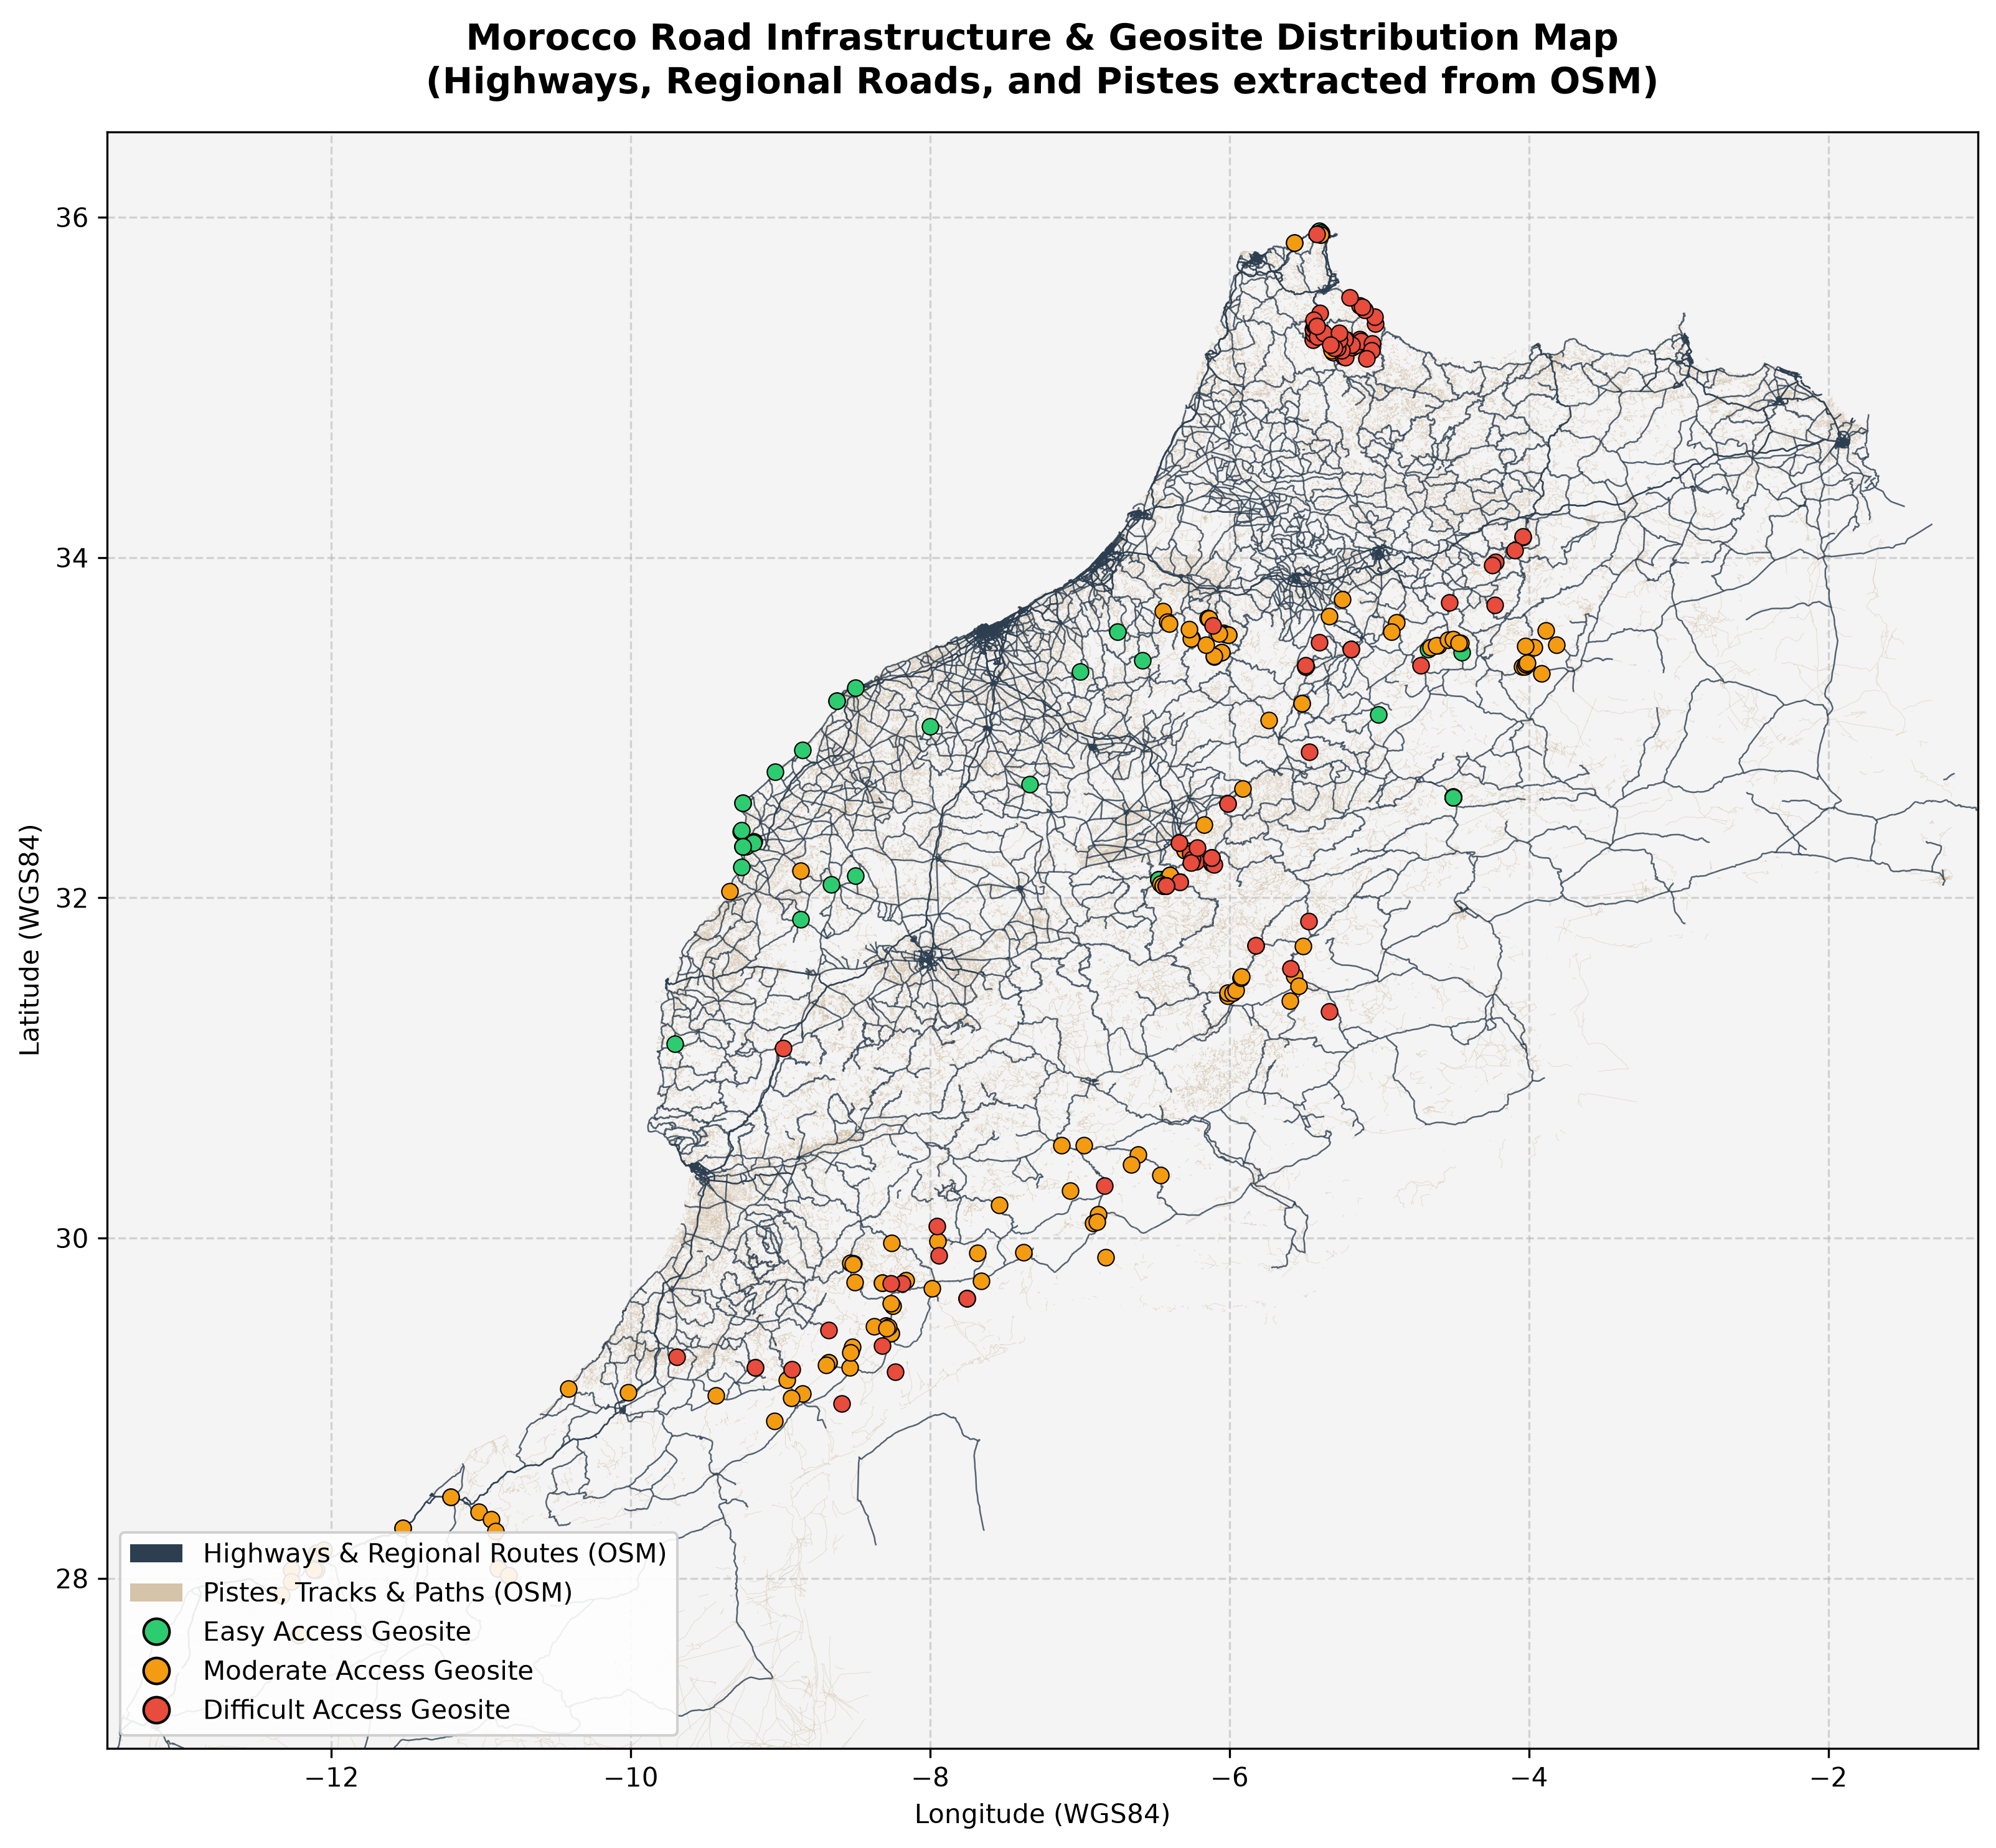
\includegraphics[width=0.45\textwidth]{map.png}
    \caption{Visual GIS Layout Layer (Before Extraction): The road networks and geosite points are mapped visually. Standard GIS tool exports only produce this layout, which cannot be directly ingested by ML models.}
    \label{fig:before_after}
\end{figure}

Table~\ref{tab:after_data} shows the clean, lossless structured data (After Extraction) generated by the tool, which is directly consumable by ML classifiers.

\begin{table}[H]
    \centering
    \caption{Extracted Tabular Feature Output (After Extraction)}
    \label{tab:after_data}
    \scriptsize
    \setlength{\tabcolsep}{2.2pt}
    \begin{tabular}{lccccc}
        \toprule
        \textbf{Geosite Name} & \textbf{Elev (m)} & \textbf{Slope ($^\circ$)} & \textbf{Soil} & \textbf{LULC} & \textbf{Dist Hwy (m)} \\
        \midrule
        Awsard panorama & 328.0 & 0.00 & 5 & 12 & 1673.6 \\
        Tadakoust gorge & 554.3 & 0.63 & 2 & 15 & 0.0 \\
        Desert mermaid & 472.0 & 0.00 & 8 & 15 & 11227.0 \\
        Bou Trou-Al Aççama & 1251.2 & 14.80 & 1 & 6 & 840.2 \\
        \bottomrule
    \end{tabular}
\end{table}

\section{Conclusion}
The generic CLI extraction tool resolves the issues of coordinate leakage, boundary overflow, and categorical corruption. By automating CRS reprojection and nearest-neighbor lookup, it bridges the gap between GIS layout maps and machine learning pipelines, ensuring 100\% data integrity and reproducibility for future research teams.

\end{document}
